\section{User Documentation}
\textit{(This section is also part of the readme.md on the weekme-github repository)} \\
\\Using \textbf{WeekMe} you can plan your next week. Not more, not less. No bloated UI nor functions you will probably never use anyway. 
How does this \textbf{awesome application} work? Hopefully it's so intuitive that any explanation is unnecessary but just in case here we give you a short introduction.

\subsection{Account}
Like in most web apps you can sign up for an account, log in and out as well as change your password and email. And of course there is also a solution in case you forget your password. 
 	\begin{figure}[H] 
		\centering 
		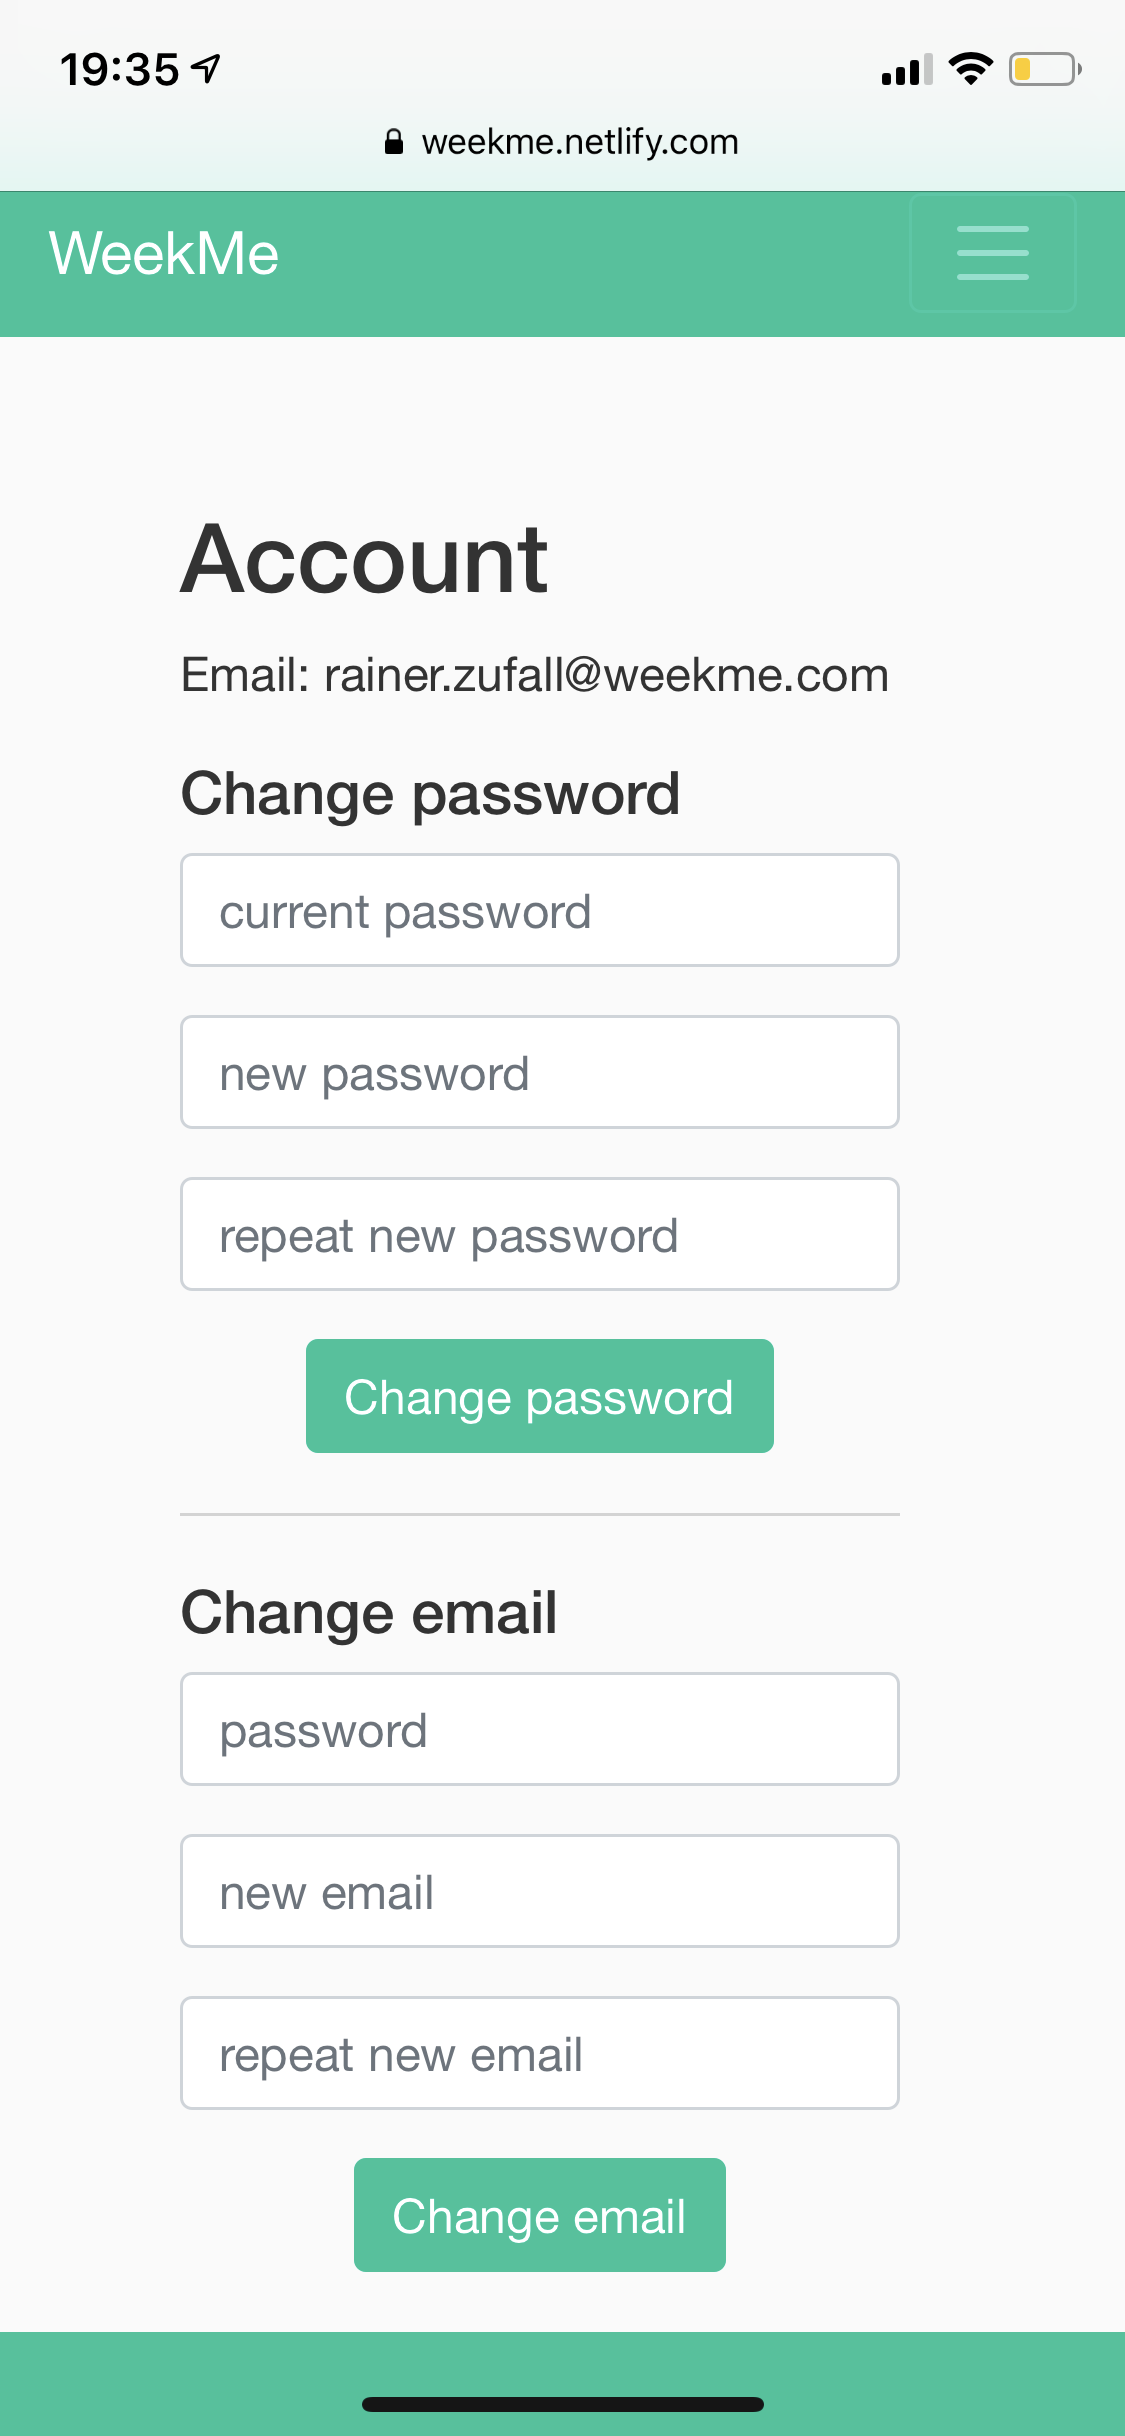
\includegraphics[height=10cm]{figures/user_docu_accounts_page.PNG}}    
		\caption{WeekMe account page on an iPhone XS}     
	\end{figure}  

\subsection{Working with tasks}
\subsubsection{The stack}
\subsubsection{Creating tasks}
\subsubsection{Editing tasks}
\subsubsection{Moving tasks}
\subsubsection{Deleting tasks}